\documentclass[12pt]{article}
\usepackage{geometry} % see geometry.pdf on how to lay out the page. There's lots.
\usepackage{natbib}
\usepackage{graphicx}
\usepackage{url}
\usepackage{color}
\geometry{a4paper} 
\usepackage{pdfpages}

%%%%%%%%%%%%%%%%
%%%%%%%%%%%%%%


\title{Supporting Information for ``Conversation, cognition and cultural evolution: a model of the cultural evolution of word order through pressures imposed from turn taking in conversation''}
\author{Se\'{a}n G. Roberts and Stephen C. Levinson}
\date{} % delete this line to display the current date

%%% BEGIN DOCUMENT
\begin{document}
\maketitle

This document contains supporting information:
\\\\
1) The R code and results for the test of the relationship between verb position and verbal affixes.  This was produced using RMarkdown.
\\\\
2) The code and results for estimating the typological distributions of languages while controlling for historical influence.  This was produced using RMarkdown.
\\\\
3) A summary of some robustness tests of the model, including the ratio of turns to conversations; populations size and noise; initial conditions; and transitions between states.
\\\\
A github repository of the data, model code, statistical code and results is available here: \url{https://github.com/seannyD/TurnTakingCulturalEvolution}.

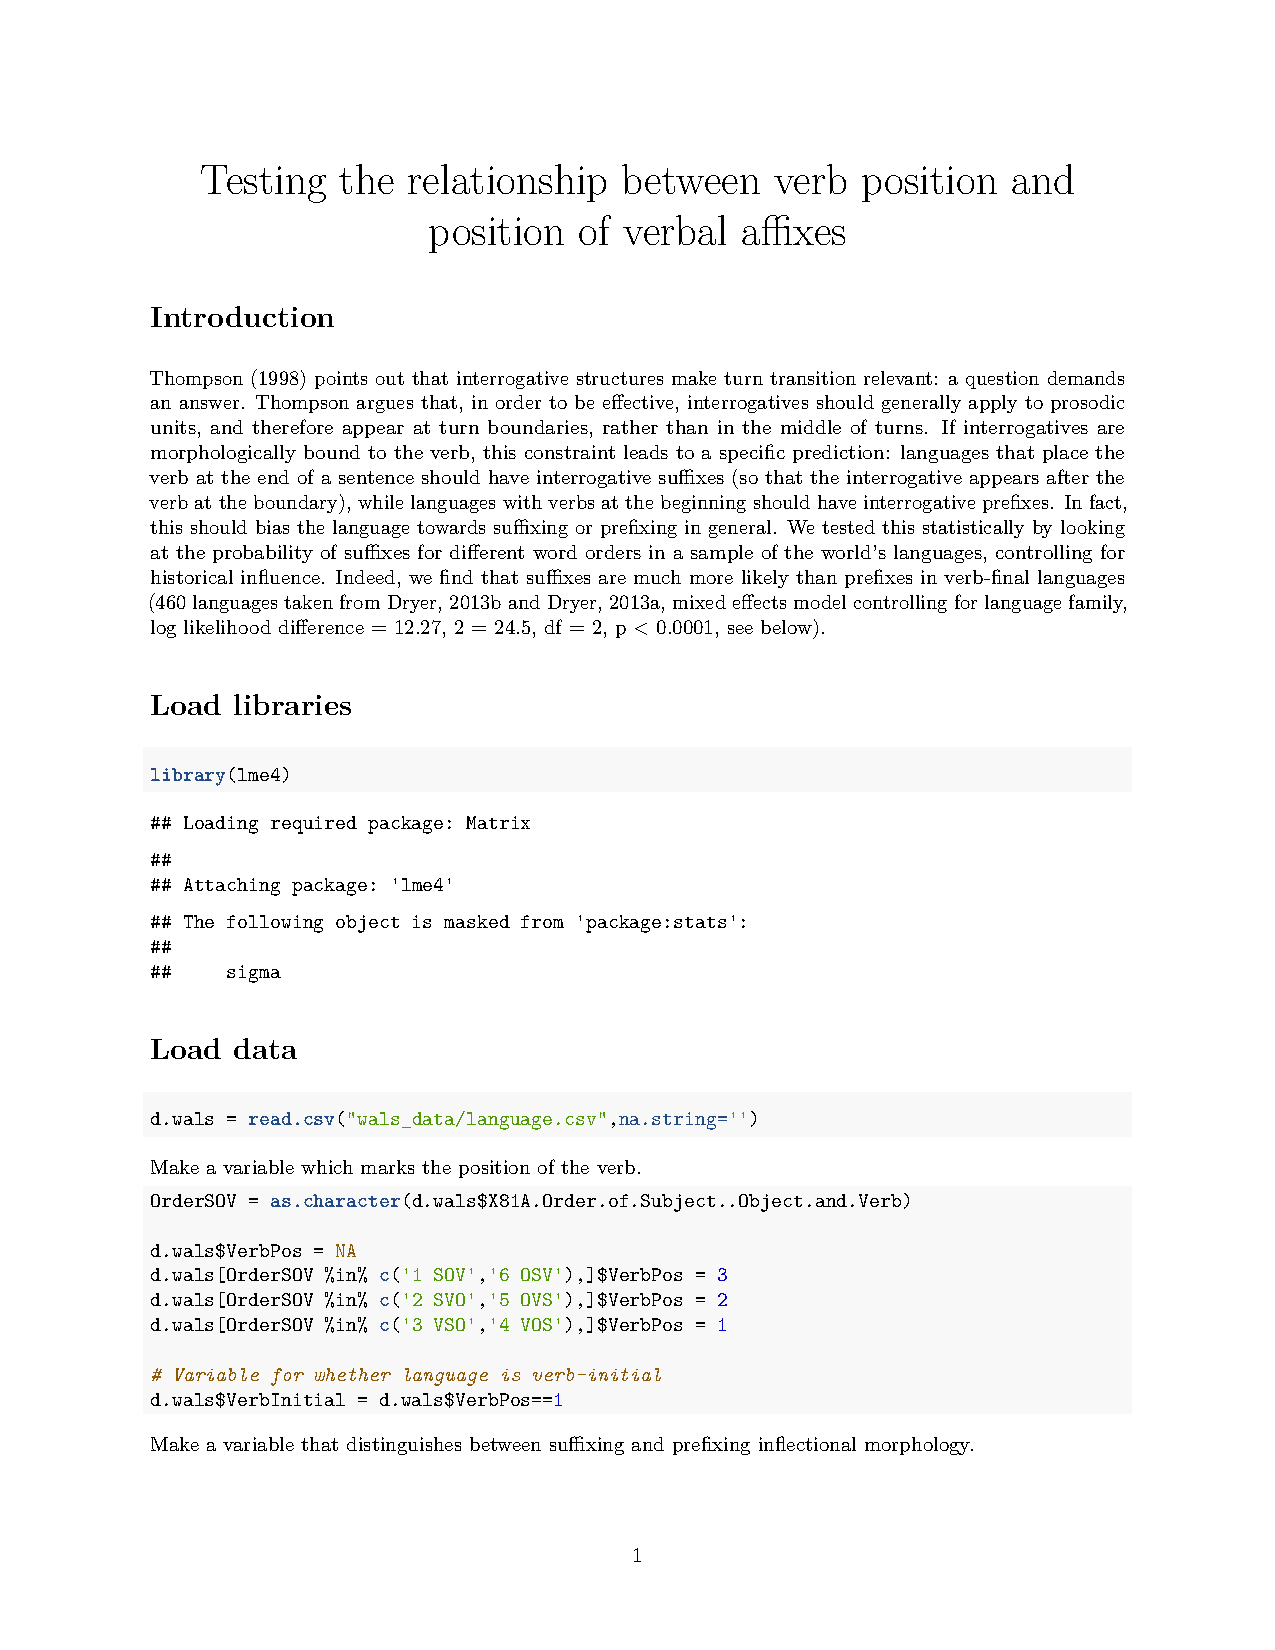
\includepdf[pages={-}]{../../EstimatesOfRealData/ThompsonInflectionalMorphologyTest.pdf}

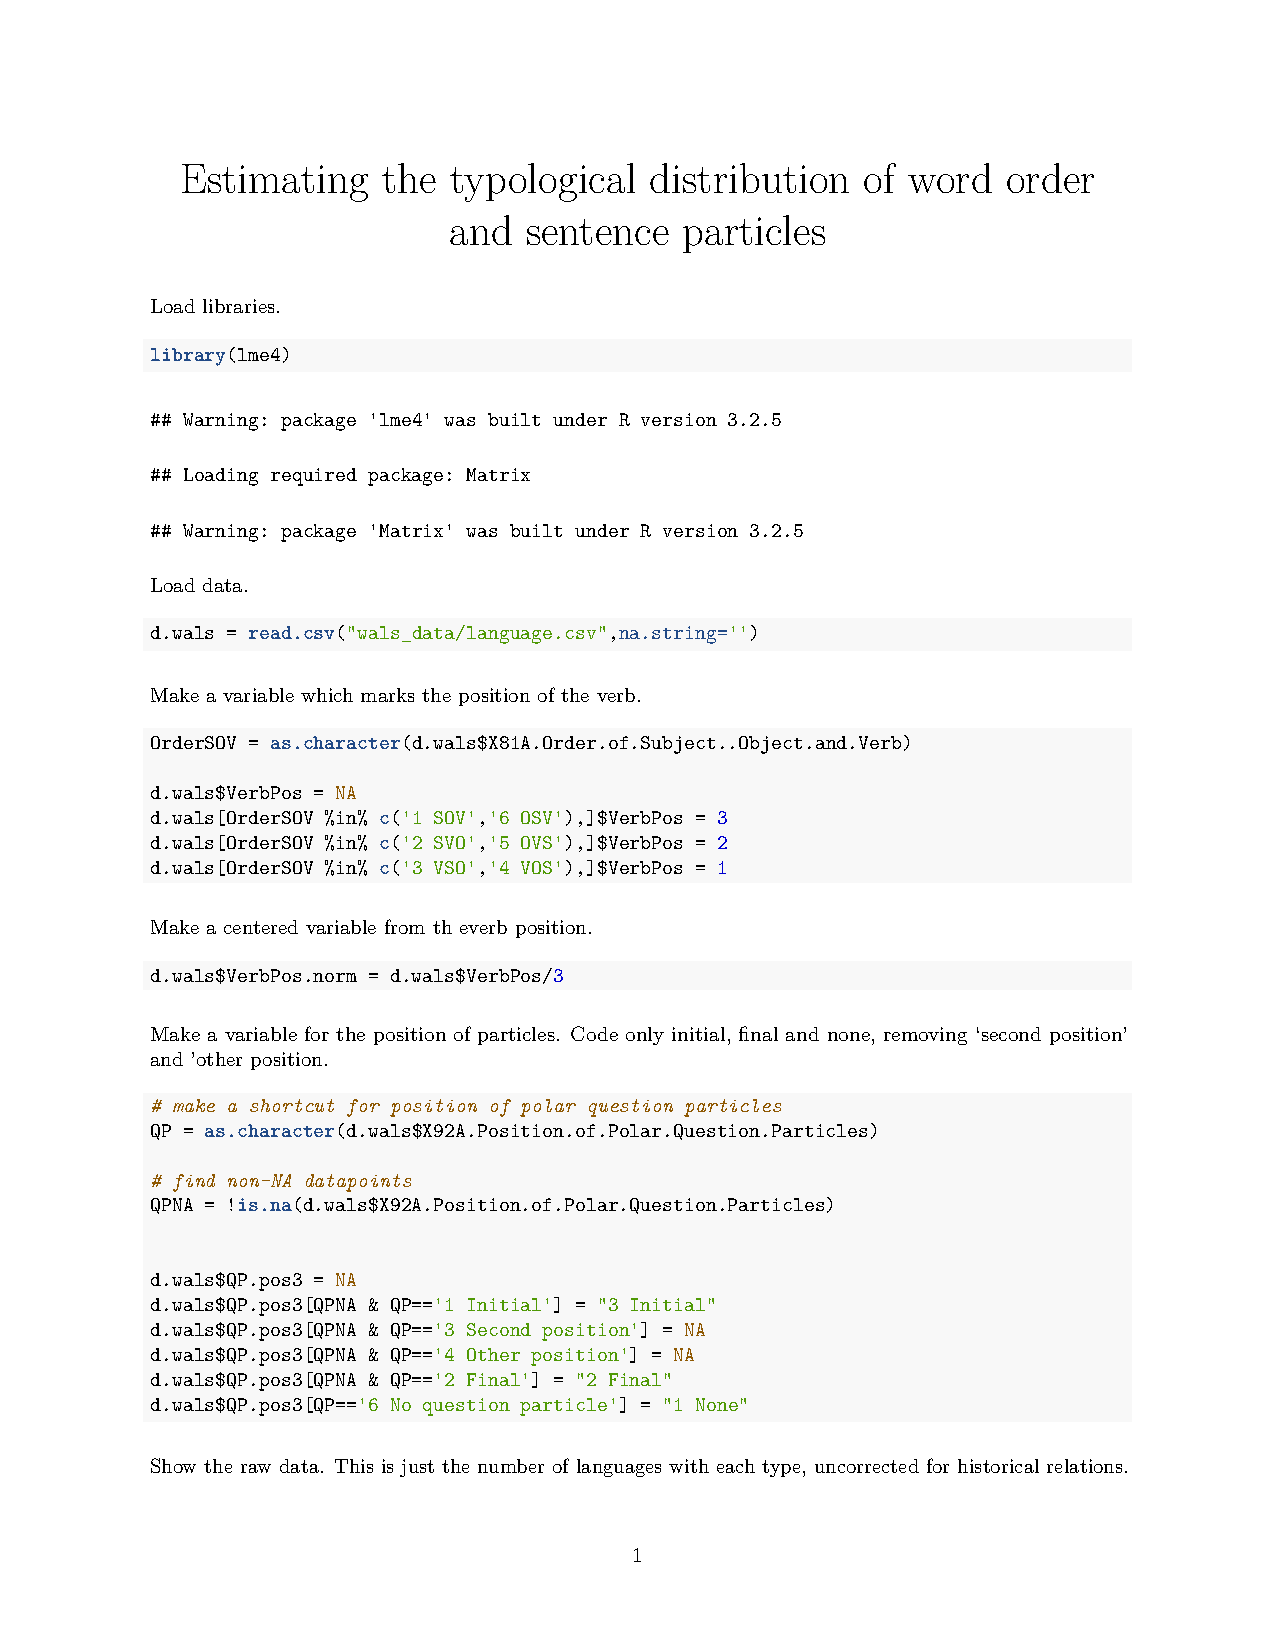
\includepdf[pages={-}]{../../EstimatesOfRealData/EstimateTypology.pdf}

\clearpage
\newpage

\section*{Model exploration}

\section{Robustness to turn taking pressure}
Figure \ref{fig:ConvTurns} shows how the distributions of word orders varies with the number of turns in each conversation.  Note that the total number of turns remains the same, only the division into conversations differs.  For each combination of $N_{conversation}$ and $N_{turns}$, 100 simulations were run ($N_{agents} = 10$, $\alpha$ = 0.1, $\beta$ = 0).  % no learning as talking).  
Even a small pressure from turn taking creates a difference in word order distributions.

\begin{figure}[htbp]
\begin{center}
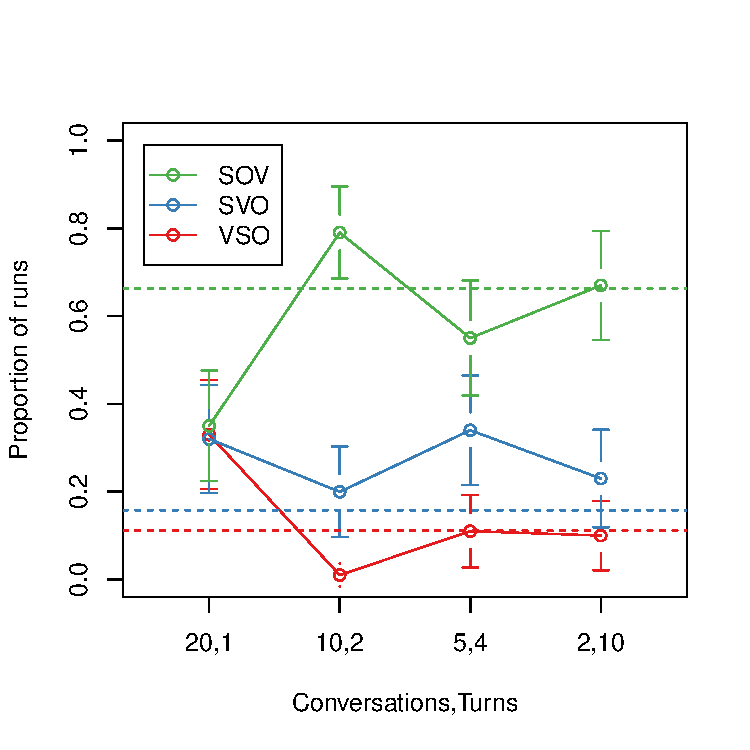
\includegraphics[width=95mm]{../images/pdf/ConvTurns.pdf}
\caption{How the distributions of word orders varies with the number of turns in each conversation.  The horizontal axis shows number of conversations and number of turns, respectively.}
\label{fig:ConvTurns}
\end{center}
\end{figure}

\clearpage
\newpage

\section{Effect of population size and noise level}

The population size and noise level parameters were explored.  Increasing both variables should make the model less susceptible to stochastic effects.  The fit of the outcome of the model was compared to the real distributions.  This was measured as the sum of the squared error between the proportion of each word order type from the model prediction and from the estimates from real data.  Figure \ref{Fig:popsizenoise} shows that the error decreases as the population size and amount of noise increases.  

The model implementation is not optimised for fast processing, so only a limited range of population sizes could be tested.  The size here is obviously very small compare, but the principles in the main results should hold.

\begin{figure}[htbp]
\begin{center}
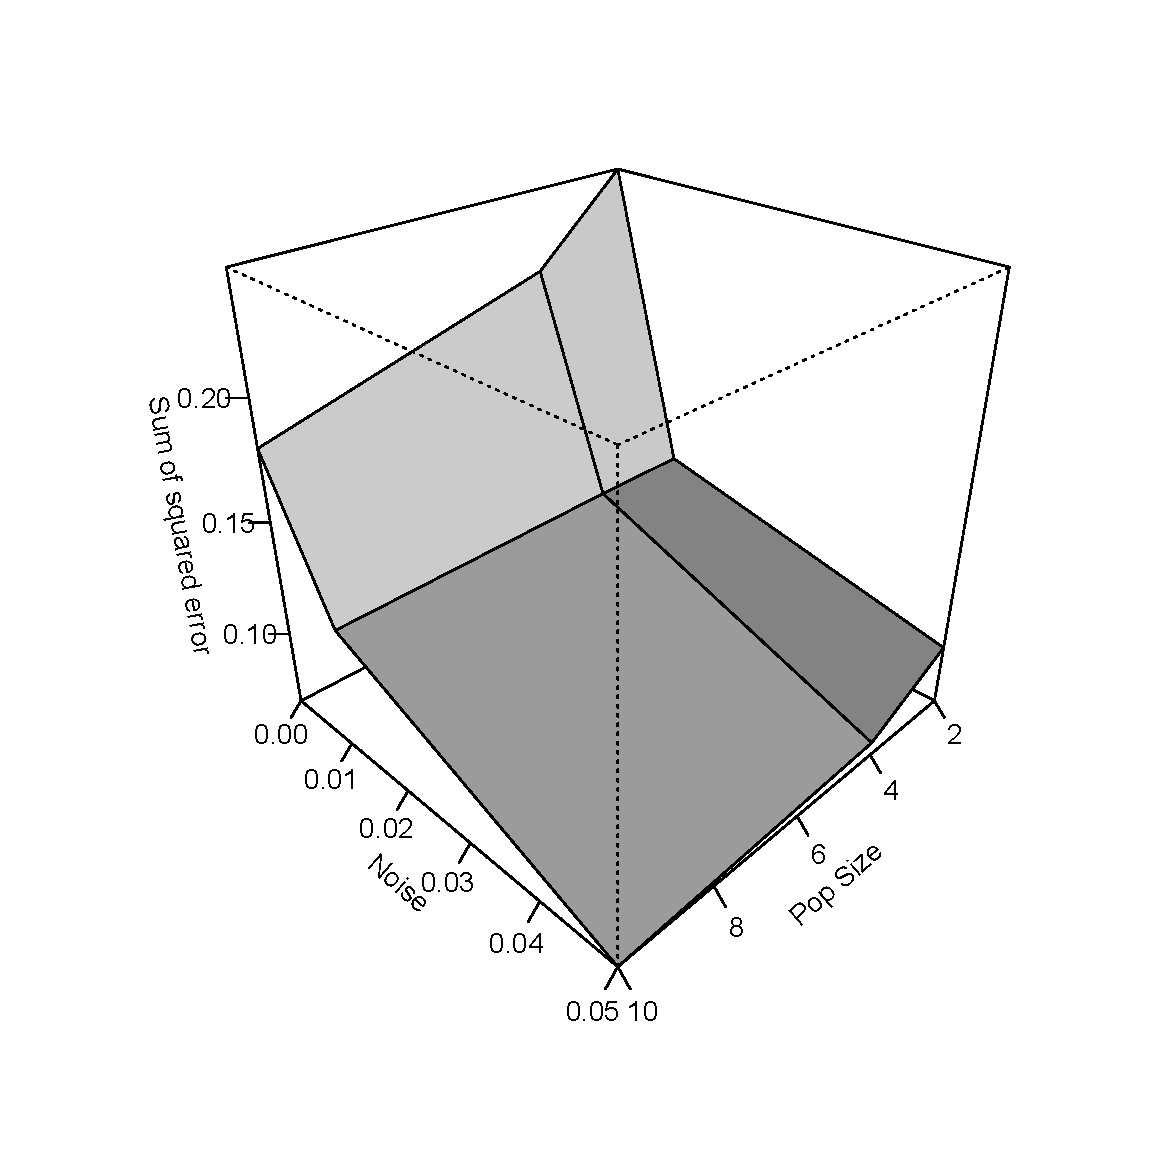
\includegraphics[width=130mm]{../images/pdf/PopSizeNoise.pdf}
\caption{How the fit of the model varies with noise and population size.}
\label{Fig:popsizenoise}
\end{center}
\end{figure}

\clearpage
\newpage

\section{Initial conditions of the model}

In the main paper, the agents in the first generation start with a uniform distribution of items in their memory, modelling a situation of no dominant word order.  We manipulated this to explore the effects of initial conditions.  For each of the basic word orders (SOV, SVO and VSO), we ran simulations where that target word order began with a higher frequency in the first generation's memory.  Simulations were run where the target word order made up 33\%, 40\%, 60\% and 80\% of  the initial distribution, with the other two types dividing the rest of the distribution evenly.  For each setting, 50 simulations were run ($n_{conversations}=1, n_{turns}=20, \beta = 0, \alpha = 0.1$).

Figure \ref{Fig:InitialConditions} below shows how the proportion of dominant word orders that arise varies with these settings.  With extreme initial conditions, the majority of runs converge on the initially biased order. However, this effect is strongest when the model is initially biased towards SOV, and weakest for an initial bias towards VSO.  If SOV makes up 80\% of the initial variants, then it goes on to dominate in 98\% of runs.  For SVO this is 80\% and for VSO it is 58\%.  That is, even when initial conditions are favour VSO order, the pressure for turn taking can reduce the probability of converging on VSO order.  The `correct' ranking of word order types is robust to any single word order being up to one third more frequent that the others (second column in figure \ref{Fig:InitialConditions}), and is most robust when starting from an SOV-biased condition (top row of figure \ref{Fig:InitialConditions}). 

This does not happen when the pressures from turn taking are removed ($n_{conversations} = 20, n_{turns} = 1$, see figure \ref{Fig:InitialConditionsNoTT}).  The only way to recover the ranking of SOV $>$ SVO $>$ VSO is to assume that initial conditions strongly favoured SOV.

\begin{figure}[htbp]
\begin{center}
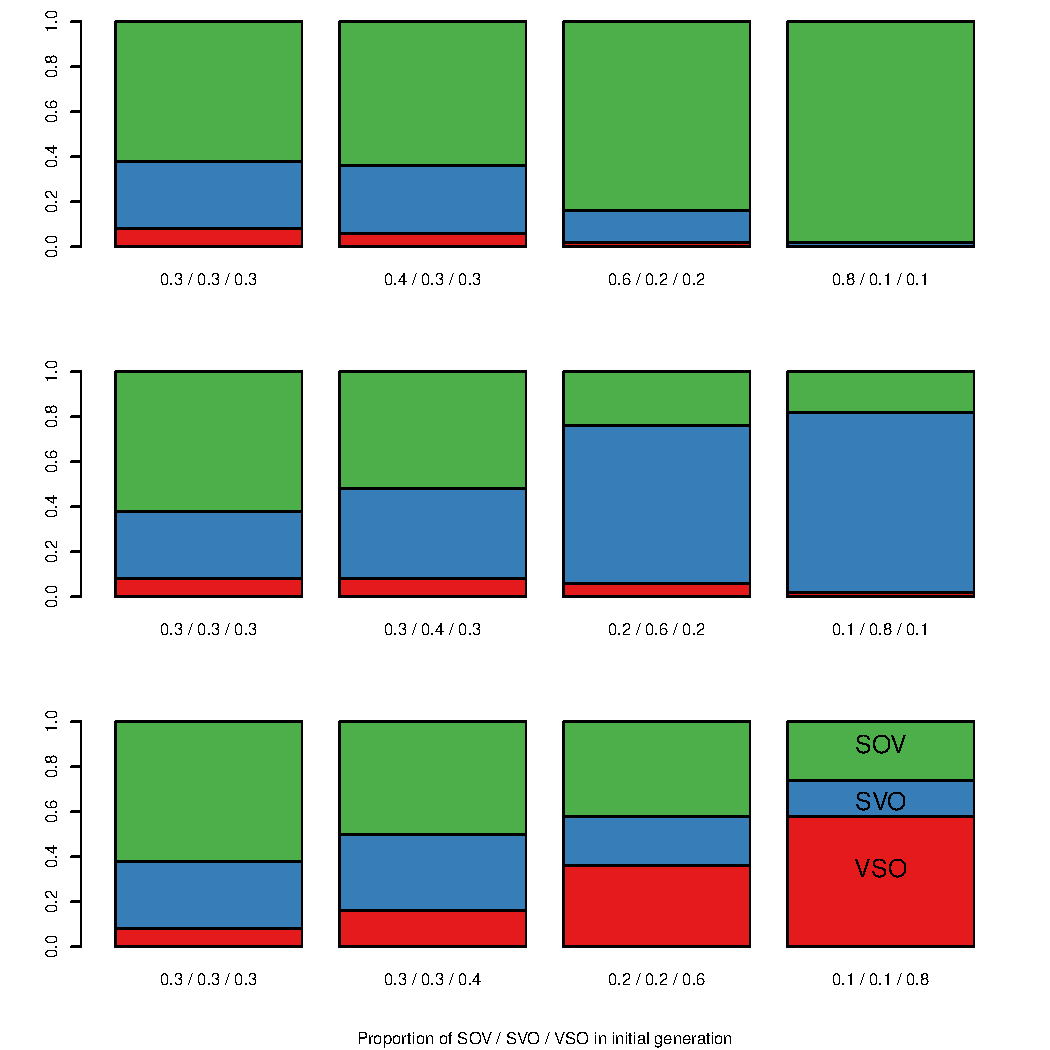
\includegraphics[width=\linewidth]{../images/pdf/InitialConditions.pdf}
\caption{Each stacked bar shows the proportion of runs converging to dominant SOV, SVO and VOS orders for a given condition.  Labels on the x axes show the initial proportion of SOV / SVO and VSO orders in the first generation.}
\label{Fig:InitialConditions}
\label{default}
\end{center}
\end{figure}

\begin{figure}[htbp]
\begin{center}
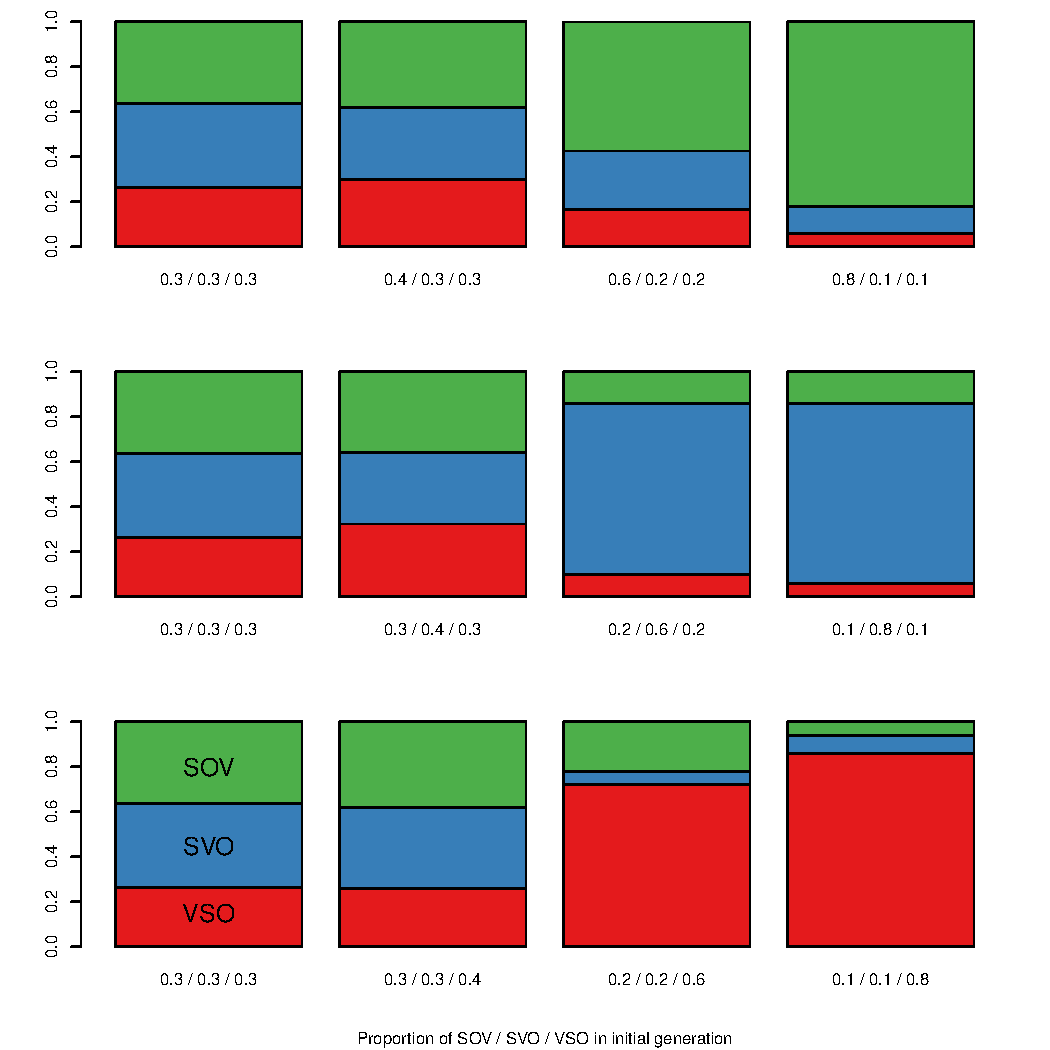
\includegraphics[width=\linewidth]{../images/pdf/InitialConditions_noTTpressure.pdf}
\caption{As above, but where the model does not have a pressure for rapid turn taking ($n_{conversations}=20, n_{turns}=1$).}
\label{Fig:InitialConditionsNoTT}
\label{default}
\end{center}
\end{figure}

\clearpage
\newpage

\section{Transitions between states}

\cite{gell2011origin} review historical changes to word order and estimate transitions between languages.  They find that word order tends to change from SOV to SVO to VSO, and suggest that languages began as SOV.  

We ran many sequences with the standard parameters, observing the dominant order at each generation, where the dominant order was the order accounting for more than 50\% of the distribution, or the previous dominant order (this was done to smooth out random fluctuations). We then explored the probability of transitions between each word order.  

\begin{table}[ht]
\centering
\begin{tabular}{rrrr}
  \hline
 & VSO & SVO & SOV \\ 
  \hline
VSO & 0.9803 & 0.0080 & 0.0085 \\ 
  SVO & 0.0027 & 0.9872 & 0.0068 \\ 
  SOV & 0.0014 & 0.0033 & 0.9919 \\ 
   \hline
\end{tabular}
\caption{Transition probabilities between dominant word orders within a run of the model.  Columns = from, rows = to, e.g. SVO changes to SOV 0.68\% of the time.  Each row sums to 1.}
\end{table}

The most common pattern is to stay with the existing dominant variant, accounting for about 98\% of transitions.  SOV is about twice as likely to transition to SVO than VSO, in line with \citeauthor{gell2011origin}'s order. However, SVO is about twice as likely to transition to SOV than to VSO.  Also, VSO is about equally likely to transition to either of the other types.  In summary, the model transitions do not fit well with those outlined in the linguistic literature on historical change.

However, the mechanism of change discussed in \citeauthor{gell2011origin} is grammaticalisation, rather than drift, and we don't have any model of interactions between grammatical structures.  They also suggest that word order distributions have not reached a stable equilibrium, while in our study we assume that they have.  Our model is more focussed on the stage of language evolution that \cite{Scott-Phillips_Kirby_2010} call ``cultural evolution'' - the initial emergence of salient features of language such as dominant word order, rather than ``historical change'' which describes more recent changes between dominant states.  In this case, an alternative view of our model is as an explanation of the starting conditions which feed into the historical changes described in \citeauthor{gell2011origin}.  That is, languages are likely to go from no fixed word order to having SOV order.  Indeed, Our model does not have any additional mechanisms such as grammaticalisation which would cause transitions between dominant word orders after the initial convergence.

\subsection{Model with particles}

The table below gives the transition probabilities for the model with optional initial or final particles, based on 1000 runs of 300 generations each ($N_{conversations}$=20, $N_{turns}$=1, $N_{agents}$ = 10, $\alpha$ = 0.1, $\beta$ = 0, $p$ = 0.5).  Numbers are proportions of generations which transition from the type in the vertical row to the type in the horizontal column (e.g. VSO transitions to VSO in 92.2\% of generations).  Generations are coded based on the most frequent order type.  Generations that have no dominant order are coded as "None".

\begin{table}[ht]
\centering
\begin{tabular}{rrrrrrrrrrr}
  \hline
 & None & VSO & SVO & SOV & VSOX & SVOX & SOVX & XVSO & XSVO & XSOV \\ 
  \hline
None & 0.264 & 0.042 & 0.073 & 0.090 & 0.052 & 0.086 & 0.103 & 0.075 & 0.095 & 0.119 \\ 
  VSO & 0.029 & 0.929 & 0.004 & 0.005 & 0.005 & 0.004 & 0.006 & 0.004 & 0.006 & 0.008 \\ 
  SVO & 0.017 & 0.002 & 0.963 & 0.003 & 0.001 & 0.003 & 0.003 & 0.003 & 0.003 & 0.003 \\ 
  SOV & 0.010 & 0.000 & 0.001 & 0.978 & 0.001 & 0.001 & 0.002 & 0.001 & 0.002 & 0.003 \\ 
  VSOX & 0.017 & 0.002 & 0.001 & 0.003 & 0.957 & 0.003 & 0.004 & 0.004 & 0.004 & 0.004 \\ 
  SVOX & 0.014 & 0.001 & 0.002 & 0.002 & 0.001 & 0.970 & 0.002 & 0.002 & 0.002 & 0.002 \\ 
  SOVX & 0.010 & 0.001 & 0.001 & 0.002 & 0.001 & 0.001 & 0.980 & 0.001 & 0.002 & 0.002 \\ 
  XVSO & 0.011 & 0.001 & 0.003 & 0.002 & 0.001 & 0.002 & 0.002 & 0.975 & 0.002 & 0.002 \\ 
  XSVO & 0.007 & 0.001 & 0.001 & 0.001 & 0.001 & 0.001 & 0.001 & 0.001 & 0.984 & 0.002 \\ 
  XSOV & 0.006 & 0.000 & 0.001 & 0.001 & 0.000 & 0.001 & 0.001 & 0.001 & 0.001 & 0.987 \\ 
   \hline
\end{tabular}
\end{table}

\bibliographystyle{apalike}
\bibliography{/Users/sgroberts/Documents/PhD/Biblography}

\end{document}